% !TeX root = 场论与凝聚态.tex

\section[The Origin of $\mathrm{i} 0^{+}$]{Where comes the $ \mathrm{i} 0^{+}$: a Non-Perturbative Interpretation}
Unitarity and locality plays an unreplaceable role in QFT and a lot of deep conclusion can be gained directly from these two properties, without the need of calculation of specific model.

In QFT, we compute something like
\begin{equation}
  \bra{\phi} \cdots \ket{\psi}, \ \text{or}\ \int_{\text{b.c.}} \mathcal{D} (\square)  \exp \left( \cdots \right) ,
\end{equation}
respectively in operator and path integral methodology, and b.c. stands for boundary condition.

In condensed matter, the experiment are done by disturbing a ground state, and the system would decay from excited state to ground state eventually, thus (near $T \sim 0$) what we usually compute is
\begin{equation}
   \bra{0} \cdots \ket{0}.
\end{equation}
And in particle phys., after performing LSZ reduction, any initial or final state would be turned into creation/annihilation operators acting on a ground state, thus, similarly, we compute
\begin{equation}
  \bra{\phi}\cdots \ket{\psi} \to  \bra{0} O^{\dagger}_{\phi} \cdots O_{\psi}\ket{0}.
\end{equation}

Furthermore, it seems that we need to get the wave function of ground state ,which would be extremely hard in any theory with interaction, however, we do not actually need to do so. The following of this section would explain it in detail.

A typically computation would be in the form of
\begin{equation}
  \bra{\phi} \mathrm{e}^{ \mathrm{i} t_f H} \mathrm{e}^{\mathrm{i}  t_i H} \ket{\psi},
\end{equation}
where the initial and final time are set at $-\infty$ and $+\infty$ for the reason that the time interval of a physical process would be greatly smaller that of an experiment.

\paragraph{Operator}
A commonly used trick is to make a substitution of $\mathrm{e}^{- \mathrm{i} \Delta t H} \to \mathrm{e}^{- i\Delta t H \left( 1- \mathrm{i}  0^{+} \right) }$ in time evolution. \footnote{It is no longer unitary, but that's what we want.}
Let's check its property in two cases: finite time and infinite time.
When $\Delta t$ is finite, there's nothing abnormal. When $\Delta t \to  + \infty$, a factor of exponentially suppress appears, yet except for states whose $H = 0$. This term would effectively become $\ket{0} \bra{0}$ or $\sum_i \ket{0_{i}} \bra{0_{i}}$ when $H \ket{0} = 0$.

If, unfortunately, the experiment time isn't literally infinite, the $0^{+}$ have to be
\begin{equation}
  0^{+} \sim \frac{1}{\text{experiment time}}\quad (\text{or relaxation time } t).
\end{equation}

In Green function, this projection to ground state is included by substitution of
\begin{equation}
   \begin{aligned}
     \omega \to \left( 1 + \mathrm{i} 0^{+} \right) \omega \quad &\text{(time ordered)}
     \\
     \omega \to \omega + \mathrm{i}  0^{+}\quad &\text{(retarded)}
   \end{aligned}.
\end{equation}

\paragraph{Path Integral}
After a substitution of $H \delta t \to H \left( 1-\mathrm{i}  0^{+} \right) \delta t$, we obtain
\begin{equation}
  \int_{\text{No b.c.}} \mathcal{D} p \, \mathcal{D} x \, \exp \left( \frac{\mathrm{i} }{\hbar} \int \left[ p\, \mathrm{d} x - H \left( 1-\mathrm{i} 0^{+} \right) \, \mathrm{d} t\right]  \right) .
\end{equation}

\paragraph{Wick Rotation}
In the process given above, we have \emph{rotated} the trajectory of $t$ from the real axis to another line through the original point with a small angle $0^{+}$. A generalization of this trick is to choose a integral contour along the imaginary axis, which is called \emph{Wick rotation}. 
It can be shown that, in principle, if we know all observables along the $z = -\mathrm{i} \tau$ axis, all observables on real time can be recovered to the spirit of analytical continuation.
\begin{figure}[h]
  \centering
  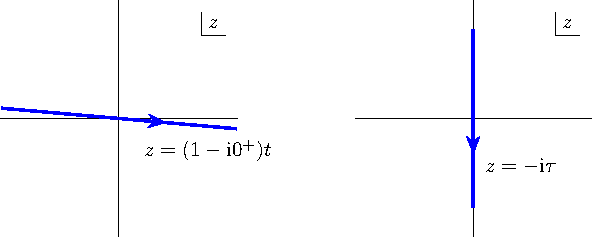
\includegraphics{figures/wick_rotation.pdf}
  \caption{Wick rotation}
\end{figure}
Under this, the expression of path integral becomes 
\begin{equation}
  \int \mathcal{D} \pi \, \mathcal{D} \phi \, \exp \left[ \frac{\mathrm{i} }{\hbar} \int \mathrm{d} \tau \, \mathrm{d} ^{3} r \left( \pi \mathrm{i}  \partial_{t} \phi - \mathcal{H} \right)  \right] .
\end{equation}
This formalism is also called \emph{Euclidean field theory} or \emph{imaginary time} path integral.

The name ``Euclidean'' field theory comes from the fact that after completing the integration on $\pi$ of a free field, we would find the term on the exponential becomes
\begin{equation}
  \mathcal{L}_{\text{Euclidean}}\sim \left( \partial_{t} \phi \right) ^{2} + \left( \partial_{\vec{r}} \phi \right) ^{2} + \phi^{2},
\end{equation}
instead of the Lagrangian density in Minkovski spacetime, whose form is typically 
\begin{equation}
  \mathcal{L}_{\text{Minkovski}} = \left( \partial\phi \right) ^{2} - m^{2} \phi^{2} = \left( \partial_{t} \phi \right) ^{2} - \left( \partial_{\vec{r}} \phi \right) ^{2} - m^{2} \phi^{2}.
\end{equation}
The iconic minus signs from Minkovski metric were eliminated after Wick rotation as if it morphed into a field living in Euclidean space.


\section{Dualities of QFT and Stat. Mech.}
\subsection{Partition Function as Path Integral}
In statistic mechanics, we compute the partition functions of fields,
\begin{equation}
  \mathcal{Z} = \sum_{s} \mathrm{e}^{-\beta E_{s}} = \sum_{s} \mathrm{e}^{-\beta \int \mathrm{d} \vec{r} \, \mathcal{H}},
\end{equation}
which is easy to compute in classical statistic mechanics where $\hbar = 0$, i.e., all operators commute.

However, in quantum cases, the calculation of
\begin{equation}
  \mathcal{Z} = \Tr \left( \mathrm{e}^{- \beta H} \right) = \Tr \left( \mathrm{e}^{-\beta \int \mathrm{d}^{d} \vec{r} \, \mathcal{H} } \right) 
\end{equation}
becomes impossible, because energy eigenstates are non-local and the eigenvalues of Hamiltonian are hard to find.
To solve this, we consider the $\mathrm{e}^{-\beta H}$ as a product of a series of $\mathrm{e}^{-\beta \epsilon}$. By analogy, we insert a completeness relation of momenta and field operators in between each of them. Whereby, we get
\begin{equation}
  \mathcal{Z} = \prod_{\vec{r}, t}^{} \left( \frac{1}{2\pi\hbar} \int \mathrm{d} \pi_{\tau + \frac{\delta \tau}{2}, \vec{r}} \, \mathrm{d} \phi_{\tau, \vec{r}}  
  \right)  
  \exp \left[ \frac{1}{\hbar} \int_{0}^{\beta\hbar} \mathrm{d}\tau \,\mathrm{d} ^{d} r\, \left( \pi \mathrm{i}  \partial_{\tau} \phi - \mathcal{H}\left( \pi, \phi \right)  \right) \right] 
\end{equation}
This expression is local
\footnote{
  It is of full necessity to indicate that a theory with locality means it is defined locally and does not have to live in $\mathbb{R}^{d} \times \mathbb{S}^{1}$ (or $\mathbb{R}^{d} \times  \mathbb{R}^{1}$).
}
in space``time'', with the cost of introducing an additional dimension on $\mathbb{S}^{1}$ (note that calculating trace implies that initial state and final state are the same thus this dimension is rolled up.) \textbf{We have clearly verified that a $d$-dim space statistic field theory is close related to a QFT in $(d+1)$-dim spacetime.}

\begin{itemize}
  \item When $\beta \to \infty$, it becomes the Euclidean QFT.
  \item When $\hbar \to  0$,
  \begin{equation}
    \frac{1}{\hbar} \int^{\hbar \beta} \mathrm{d} \tau \, \left( \square \right) \to \beta \frac{\partial }{\partial \tau} \int \mathrm{d} \tau \, \left( \square \right)  \to  \beta \left( \square \right) ,
  \end{equation}
  hence it goes back to classical case.
\end{itemize}

Additional compatibilities can be intuited directly from the form of path integral mopped up the momentum $\pi$, listed as follows:
\begin{equation*}
  \begin{matrix}
      d\text{-space quantum Stat. Mech.}\\
      \Updownarrow \\
      (d+1) \text{-spacetime QFT}\\
      \Updownarrow \\
      (d+1) \text{-space classical Stat. Mech.}
  \end{matrix}
\end{equation*}

The statistic field theory integrated out momenta is
\begin{equation}
  \mathcal{Z} = \int \mathcal{D} \phi  \, \exp\left[ - \int \underbrace{\mathrm{d} \tau \, \mathrm{d} ^{d} r}_{\mathrm{d} ^{d+1} r \text{ in } \Sigma \times \mathbb{S}^{1}}\, \left( \frac{\left( \partial_{\tau} \phi \right) ^{2}}{2} + \frac{\left( \partial_{\vec{r}} \phi \right) ^{2}}{2} + V\left( \phi \right)  \right) \right] 
\end{equation} 
which can be rewritten as
\begin{equation}
  \mathcal{Z} = \int \mathcal{D} \phi \, \exp \left[ - \int \mathrm{d} ^{d+1} r \, \left( \frac{\left( \partial_{\tau} \phi \right) ^{2}}{2} + \frac{\left( \partial_{\vec{r}} \phi \right) ^{2}}{2} + V\left( \phi \right)  \right)  \right] .
\end{equation}
It can be reinterpreted as classical stat. mech. in $(d+1)$-space, whose, however, $\tilde{\beta}$ has no physical reflections.

